% !TEX root = ../main.tex
\section{Experience Result}

\begin{frame}{Experience Result}
  \begin{columns}
    \begin{column}{0.4\textwidth}
      \begin{block}{Loss function:}
        - Optimizer: torch.optim.Adam

        - Loss after 10 epochs (4140 batch) in figure \ref{fig:loss}
      \end{block}
      \begin{block}{Accurancy}
        - Accurancy \(\approx\) 80\%
      \end{block}
    \end{column}{}
    \begin{column}{0.6\textwidth}
      \begin{figure}
        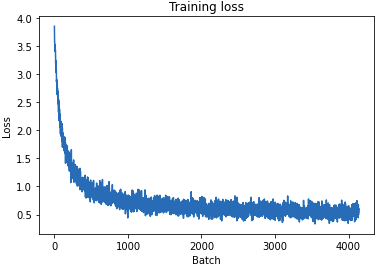
\includegraphics[width=0.8\textwidth]{figure/loss.png}
        \caption{Training loss}
        \label{fig:loss}
      \end{figure}
    \end{column}
  \end{columns}
\end{frame}

\begin{frame}{Experience Result}
  \begin{block}{Compare with other models in article}
    \begin{table}
     \begin{tabular}{|c | c|} 
     \hline
     \textbf{Model} & \textbf{Accurancy} \\ [0.5ex] 
     \hline\hline
     M3 & 56.12\% \\ 
     \hline
     M5 & 63.43\% \\
     \hline
     M11 & 69.07\% \\
     \hline
     M18 & 71.68\% \\
     \hline
     M34 & 63.47\% \\ [1ex] 
     \hline
    \end{tabular}
    \caption{Accurancy of other model (Dataset: UrbanSound8k)}
    \end{table}
  \end{block}
\end{frame}